\paragraph{Sơ đồ tuần tự Luồng Đàm thoại trực tiếp với AI bằng giọng nói}

Luồng này mô tả phiên voice chat sau khi client đã join LiveKit room. Voice Agent trong Chatbot Service nhận audio, đọc metadata từ participant, resolve persona để cập nhật DynamicTTS, gọi công cụ RAG khi câu hỏi liên quan pháp luật hoặc tài liệu cá nhân, sau đó phát audio phản hồi qua LiveKit.

\begin{figure}[H]
\centering
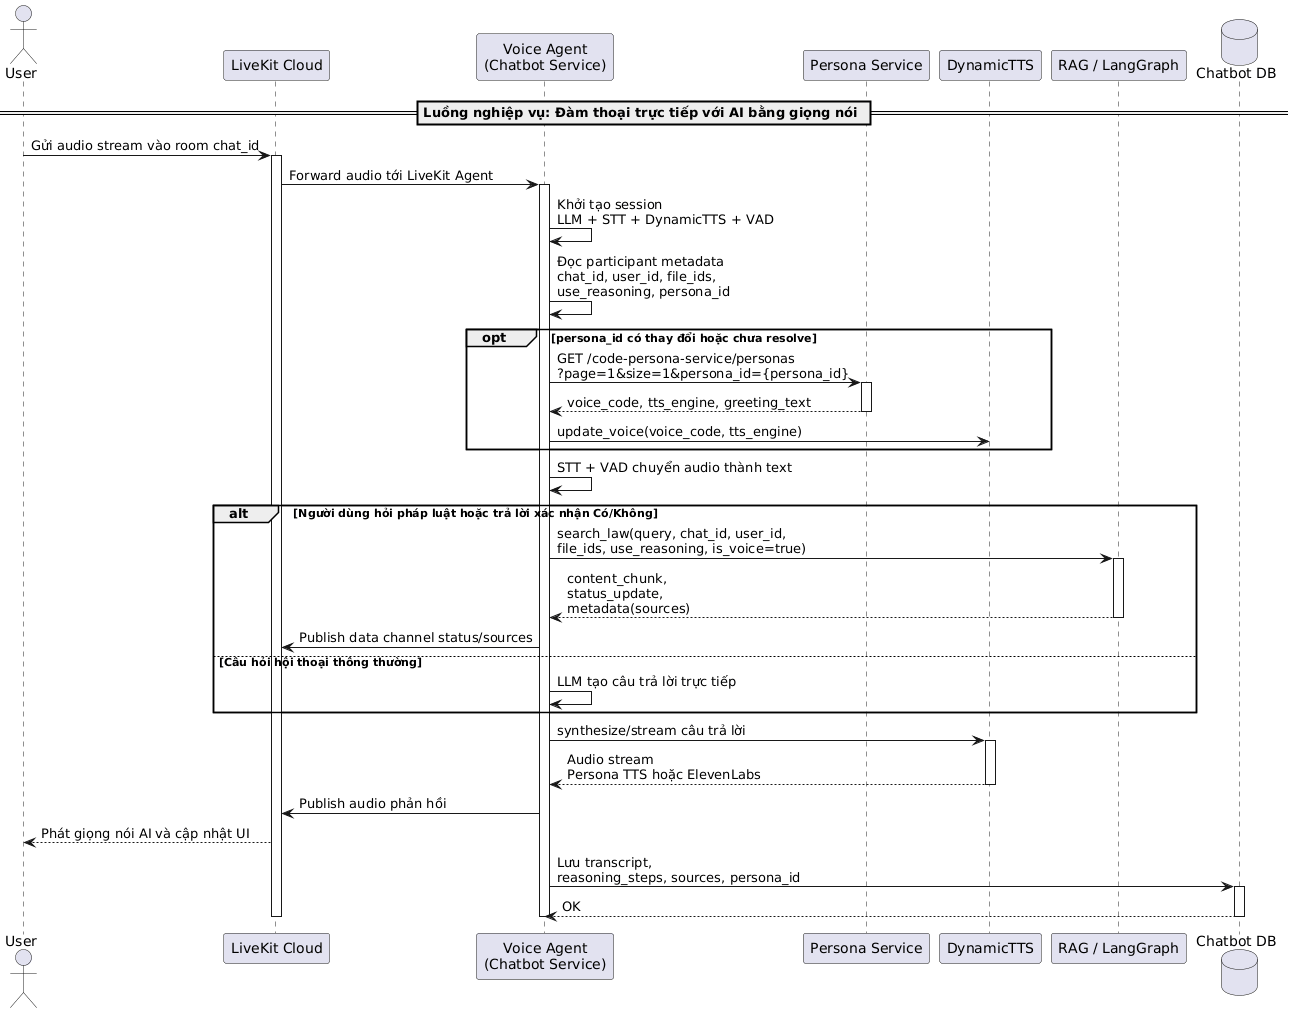
\includegraphics[scale = 0.18]{contents/Sequence/UML-Sequence-UserVoiceChatWithAi.png}
\caption{Sơ đồ tuần tự Luồng Đàm thoại trực tiếp với AI bằng giọng nói}
\end{figure}

\subparagraph{Các thành phần tham gia}

\begin{table}[H]
\centering
\renewcommand{\arraystretch}{1.3}
\begin{tabular}{|l|l|p{5cm}|}
\hline
\textbf{Thành phần} & \textbf{Phân loại} & \textbf{Vai trò trong hệ thống} \\ \hline
User & Actor & Người dùng nói chuyện trực tiếp với AI. \\ \hline
LiveKit Cloud & External Service & Chuyển tiếp audio và data channel giữa client và Voice Agent. \\ \hline
Voice Agent & Component & Xử lý STT/VAD, gọi tool RAG, publish trạng thái và lưu transcript. \\ \hline
Persona Service & Microservice & Cung cấp \texttt{voice\_code}, \texttt{tts\_engine} và thông tin persona. \\ \hline
DynamicTTS & Component & Chọn TTS theo engine hiện tại: Persona TTS qua API OpenAI-compatible hoặc ElevenLabs. \\ \hline
RAG / LangGraph & AI Pipeline & Tra cứu pháp luật, tài liệu cá nhân và sinh trạng thái reasoning. \\ \hline
Chatbot DB & Database & Lưu transcript, reasoning steps, sources và persona. \\ \hline
\end{tabular}
\caption{Các thành phần tham gia luồng đàm thoại trực tiếp với AI}
\end{table}

\subparagraph{Mô tả chi tiết}
\begin{itemize}
\item Voice Agent nhận metadata từ LiveKit participant gồm \texttt{chat\_id}, \texttt{user\_id}, \texttt{file\_ids}, \texttt{use\_reasoning} và \texttt{persona\_id}.
\item Khi \texttt{persona\_id} thay đổi hoặc chưa được resolve, agent gọi public persona endpoint để lấy \texttt{voice\_code} và \texttt{tts\_engine}, sau đó gọi \texttt{DynamicTTS.update\_voice}.
\item STT/VAD chuyển audio thành text. Nếu câu hỏi liên quan pháp luật hoặc là phản hồi xác nhận, agent gọi tool \texttt{search\_law}.
\item Tool RAG gọi \texttt{generation\_stream(..., is\_voice=true)} và trả về \texttt{status\_update}, \texttt{content\_chunk}, \texttt{metadata}; status và sources được gửi về UI qua data channel.
\item Câu trả lời được chuyển thành audio bằng DynamicTTS và phát lại qua LiveKit, đồng thời transcript được lưu vào Chatbot DB.
\end{itemize}
